\chapter{Deep Dive into the Application}\label{chap:deep-dive-app}

This chapter gives a detailed, implementation-focused look at the Django application for experimental data management. 
The system is built with a layered architecture that separates business rules, storage access, background processing, and presentation. 
It connects to an external identity provider (Authentik via OIDC), stores both raw and derived data in an S3-compatible object store (Ceph RGW/MinIO), 
and uses Redis Queue (RQ) for asynchronous tasks.
The following sections describe the data model, information flows, metadata handling, NeXus file construction, storage gateway, 
background jobs, API and user interface, the in-app security model, and performance and scalability aspects.

%%%%%%%%%%%%%%%%%%%%%%%%%%%%%%%%%%%%%%%%%%%%%%%%%%%%%%%%%%%%%%%%%%%%%%%%%%%%%%%%%%%%%

\section{Domain model and data flow}\label{sec:domain-dataflow}

\paragraph{Entities.}
The application organises information into four main building blocks, each represented by a Django model:

\begin{itemize}
	\item \textbf{Project}: this is the top-level container, for example \emph{NFFA\_DI}. 
	Each project has a human-readable \texttt{name} and a machine-friendly \texttt{slug} 
	(a simplified version of the name, produced automatically by a local \texttt{slugify} helper). 
	The slug is guaranteed to be unique so that it can safely be used in URLs and bucket names.
	
	\item \textbf{Proposal}: a proposal belongs to exactly one project and is uniquely identified by the pair 
	(\texttt{project}, \texttt{number}). In addition to the proposal number, it stores information such as the 
	principal investigator (\texttt{pi\_name}), the proposal date, a free-text \texttt{description}, and the user who created it. 
	Each proposal also owns exactly one S3 bucket (\texttt{bucket}) where its raw data is stored. 
	This bucket name is created automatically the first time the proposal is saved: 
	it combines the project slug and proposal number, and adds an 8-character SHA-1 hash for uniqueness, 
	prefixed with \texttt{lame-raw-} (or another prefix from settings).
	
	\item \textbf{Sample}: a sample belongs to one proposal and is uniquely identified by the pair 
	(\texttt{proposal}, \texttt{slug}). The slug is derived from the sample’s \texttt{name}. 
	Samples may also carry optional descriptive fields such as an external \texttt{identifier}, 
	a \texttt{preparation\_date}, the list of \texttt{atom\_types}, and a description of the \texttt{physical\_form}. 
	These optional details are written into README files to keep them close to the data.
	
	\item \textbf{Experiment}: an experiment belongs to one sample and is uniquely identified by the pair 
	(\texttt{sample}, \texttt{slug}). It can have a free-text \texttt{description} and optional start-time metadata. 
	Experiments group together the actual measurement files uploaded by users.
\end{itemize}

The database enforces these uniqueness rules through Django’s \texttt{Meta} constraints (\texttt{UniqueConstraint} or 
\texttt{unique\_together}), which prevents accidental duplication.  

\paragraph{Domain commands.}
To create these entities, the application does not call the models directly.  
Instead, it uses command functions in \texttt{domain/commands.py}, such as \texttt{create\_proposal}, 
\texttt{create\_sample}, and \texttt{create\_experiment}.  
These commands wrap several steps into one unit of work:

\begin{enumerate}
	\item \textbf{Friendly validation}: before writing, they check if an entity with the same identifiers already exists, 
	and if so, raise a \texttt{ValidationError} with a clear message (avoiding generic database errors).
	\item \textbf{Safe database write}: the actual insert happens inside a transaction. 
	If two requests collide, the code re-checks after catching an \texttt{IntegrityError} 
	so that the user still gets a meaningful error message instead of a crash.
	\item \textbf{Bucket provisioning}: when a proposal is created, the corresponding bucket is created (or confirmed to exist) 
	using \texttt{create\_bucket}. Calling this every time is safe, because the operation does nothing if the bucket already exists.
	\item \textbf{README writing}: immediately after creation, a README file is generated with the entity’s metadata 
	(e.g.\ project name, proposal number, sample identifier, experiment start time) and written to object storage at a standard path 
	such as \texttt{<proposal\_prefix>/README.txt}, \texttt{<sample\_prefix>/README.txt}, or \texttt{<experiment\_prefix>/README.txt}.
\end{enumerate}

In this way, each creation command leaves both the database and the storage layer in sync:  
a new row is added to the relational database, the bucket (if any) is guaranteed to exist, and a README appears in storage 
so that anyone browsing raw data can also see the associated metadata.


\paragraph{Lifecycle and flow.}
The typical sequence of actions is:

\begin{enumerate}
	\item \textbf{Creation via forms or API.} Users create projects, proposals, samples, or experiments through HTMX modals 
	(\texttt{view\_modals.py}) or the REST API. The modals call the domain commands. 
	On success, the server replies with \texttt{204 No Content} and triggers a refresh in the browser. 
	If validation fails, the modal is re-rendered with a single error block, instead of returning a generic HTTP error.
	
	\item \textbf{README writing.} Right after each entity is created, a README file is written into object storage through the storage gateway. 
	The path is predictable (\texttt{<proposal\_prefix>/README.txt}, \texttt{<sample\_prefix>/README.txt}, 
	\texttt{<experiment\_prefix>/README.txt}), and the body is generated by \texttt{services/readme.py}. 
	This way, descriptive metadata always sits next to the raw data.
	
	\item \textbf{Measurement registration and raw upload.} 
	To upload data, a user chooses the target proposal, sample, and experiment. 
	The browser then uploads the raw files directly to S3 using presigned PUT URLs from \texttt{/s3\_presign}. 
	Once the upload finishes, the browser tells the backend which S3 keys were written, together with minimal metadata 
	such as the instrument pair, user name, and a short description. This is handled by \texttt{register\_measurement()}.
	
	\item \textbf{Measurement README and background jobs.} 
	\texttt{register\_measurement()} creates a measurement-level README next to the uploaded files. 
	It also schedules background jobs: one to compute a checksum for every uploaded file, and another to convert TIFFs into NeXus 
	if the instrument pair supports it. The code makes sure that the needed buckets (RAW and mirror) exist before writing.
	
	\item \textbf{Mirroring to derived buckets.} 
	The system derives the name of a “mirror” bucket using \texttt{mirror\_bucket\_for()} 
	and creates it if it does not exist. Derived artefacts such as NeXus files are uploaded here, 
	keeping them separate from raw data. The \texttt{/ofed/} view lets users browse this mirrored namespace.
\end{enumerate}

\paragraph{Consistency and error handling.}
Domain commands always validate inputs before writing, so users get clear error messages instead of database errors.  
All writes run inside database transactions to avoid partial updates.  
If two users try to create the same entity at the same time, the code re-checks uniqueness after catching an integrity error.  
Creating buckets is always safe to call multiple times, because the storage layer ignores duplicates.  
Background jobs that compute checksums use \texttt{update\_or\_create}, so retries simply update the existing row rather than causing conflicts.

%%%%%%%%%%%%%%%%%%%%%%%%%%%%%%%%%%%%%%%%%%%%%%%%%%%%%%%%%%%%%%%%%%%%%%%%%%%%%%%%%%%%%%%%%%%%%%%%%%

\section{Metadata path}\label{sec:metadata-path}

\paragraph{TIFF ingestion.}
Most raw microscope outputs arrive as TIFF files. When a user uploads them, the system only stores the object keys immediately; 
the heavy work of reading the files is left to background workers. 
TIFF parsing happens inside the builder services (see \S\ref{sec:nexus-construction}). 
For large files, the app relies on S3’s \texttt{StreamingBody} so data can be read in chunks instead of all at once. 
Typical chunk sizes are 8–16\,MiB, which are also used in checksum calculation and ZIP streaming to avoid memory spikes.

\paragraph{Instrument metadata extraction and mapping.}
Each instrument family writes metadata into TIFF headers in its own way. 
To avoid hard-coding these differences in the code, the system uses JSON mapping files stored under \texttt{experiment\_manager/data/} 
(for example \texttt{ED\_mapping.json}, \texttt{TVIPS\_mapping.json}). 
These files describe how to translate instrument-specific keys into NeXus fields. 
The chosen instrument pair (instrument + detector) is passed from the UI (\texttt{PAIRS} in \texttt{views.py}) 
through the \texttt{register\_measurement()} call and finally into the builder.

\paragraph{Translation to NXem concepts.}
The NXem definition (NeXus for electron microscopy) expects a common structure: 
an entry node with subgroups for instrument, detector, and sample, each containing well-known fields 
such as pixel size, accelerating voltage, camera length, and dwell time. 
The mapping layer is responsible for filling this structure by translating the raw metadata. Concretely:

\begin{itemize}
	\item \emph{Source fields}: information pulled from TIFF tags (e.g.\ \texttt{ImageDescription}, \texttt{XResolution}, \texttt{YResolution}, \texttt{Software}), 
	text written into measurement README files, and extra form inputs like operator or description.
	\item \emph{Mapping}: each JSON file matches these source keys (sometimes with path expressions inside \texttt{ImageDescription}) 
	to target NeXus paths (for example \texttt{/entry/instrument/detector/exposure\_time}).
	\item \emph{Normalization}: values can be converted to consistent units (e.g.\ seconds instead of milliseconds, metres instead of nanometres), 
	cast to the right data type, and filled with sensible defaults if missing.
\end{itemize}

By moving the instrument-specific rules into data files, the builder code stays simple, reusable, and easy to test.

%%%%%%%%%%%%%%%%%%%%%%%%%%%%%%%%%%%%%%%%%%%%%%%%%%%%%%%%%%%%%%%%%%%%%%%%%%%%%%%%%%%%%%%%%%%%%%%%%%%%

\section{NeXus construction}\label{sec:nexus-construction}

\paragraph{Responsibilities and split.}
The NeXus build process separates the code that \emph{creates} a NeXus file 
from the code that decides \emph{where and when} it should be stored:

\begin{itemize}
	\item \path{services/nexus_builders.py}: contains the low-level writers that take one TIFF file and a JSON mapping, 
	and turn them into a valid NXem tree (backed by HDF5). 
	The main functions are \path{build_nexus_from_tiff_TEM_ED(...)} and \path{build_nexus_from_tiff_TVIPS(...)}.
	
	\item \path{services/nexus.py}: handles the orchestration around storage. 
	It chooses the right builder for the selected instrument pair, finds or creates the mirror bucket, 
	manages temporary files, and uploads the finished \path{.nxs}. 
	Its main entry point is \path{build_and_upload_nexus(...)}.
\end{itemize}

\paragraph{Common scaffold (writer core).}
Both builders share a common function \path{_build_scaffold(...)} that sets up the basic NeXus file. 
It runs through the following steps:

\begin{enumerate}
	\item \textbf{Read and flatten metadata.} The first TIFF page is opened with \path{tifffile}. 
	All tags are flattened into a single dictionary with dot-separated keys. 
	If a string tag contains embedded JSON (for example TVIPS puts a JSON block inside \path{ImageDescription}), 
	it is parsed, flattened, and merged. Lists are indexed with keys like \path{foo[0].bar}.
	
	\item \textbf{Load mapping file.} A JSON mapping file (for example \path{ED_mapping.json} or \path{TVIPS_mapping.json}) 
	is read into a dictionary of \path{source_key -> nexus_dotted_path}. 
	Both \path{/} and \path{.} are accepted as separators in the paths.
	
	\item \textbf{Create root and entry.} An \path{NXroot} is created with the output file name. 
	Inside it, an \path{NXentry} is added and marked with \path{definition="NXem"}. 
	Group names use uppercase or explicit naming to satisfy NeXus validators.
	
	\item \textbf{Add sample block.} A required \path{SAMPLE} group (\path{NXsample}) is created with default values: 
	\path{name="UNKNOWN_SAMPLE"}, \path{identifier_sample="unknown_id"}, \path{physical_form="bulk"}, 
	and a boolean flag \path{is_simulation}. 
	If extra fields from the README forms are provided (see \S\ref{sec:metadata-path}), they replace the defaults: 
	\path{sample_identifier}, \path{preparation_date} (normalized to full ISO date-time), 
	\path{atom_types}, and \path{physical_form}.
	
	\item \textbf{Add coordinate system.} A \path{NXcoordinate_system} group called \path{coordinate_system_1} 
	is attached with fixed values: \path{type=cartesian}, \path{handedness=right}, \path{origin=front_top_left}.
	
	\item \textbf{Apply mapping.} For each flattened TIFF key found in the mapping, the corresponding NeXus path is created. 
	Intermediate groups are added as needed, and leaf values are stored as \path{NXfield(val)} without conversion.
	
	\item \textbf{Normalize start time.} If the mapping produced separate fields \path{start_time_date} and \path{start_time_time}, 
	they are combined into a single ISO8601 \path{start_time}. 
	If no start time is present at all, the default \path{1970-01-01T00:00:00Z} is used.
	
	\item \textbf{Embed image data.} The image is read with \path{tifffile.imread} 
	and stored under \path{image_2d} as an \path{NXdata} group with \path{signal="data"}.
	
	\item \textbf{Write extras and header dump.} Any extra fields not placed under \path{SAMPLE} are written at the \path{NXentry} level. 
	If a header dictionary is given, it is saved as a JSON \path{NXnote} called \path{hdr_metadata}.
\end{enumerate}

\paragraph{Instrument-specific population.}
After the scaffold, a small \emph{population} step adds instrument-facing structure in a uniform way. The builder selects a pair-specific helper from the registry and uses it to (i) ensure the expected NXem layout exists and (ii) attach common instrument nodes. Concretely, the helper:
\begin{itemize}
	\item guarantees the presence of an events branch \path{NXentry/measurement/events/event_data} with \path{NX_class=NXevent_data_em};
	\item creates an \path{instrument} subtree (\path{NXinstrument_em}) and, where relevant, children such as \path{ebeam_column} (\path{NXebeam_column} with \path{electron_source} \path{NXsource} and \path{filter} \path{NXfilter}), \path{detector} (\path{NXdetector}), and \path{stage} (\path{NXmanipulator});
	\item fills missing fields with neutral defaults (e.g., \path{"unknown"} for strings, numeric zeros for stage axes) using create-if-missing semantics, so values coming from the mapping or the caller are never overwritten;
	\item optionally adds a lightweight microscope-identity branch under \path{NXentry/measurement/instrument} (e.g., name, location, vendor/model/serial\_number).
\end{itemize}
Acquisition-specific quantities (such as exposure time, pixel size, beam voltage, trigger mode) are intentionally supplied by the JSON mapping rather than hard-coded here. Adding support for a new instrument means contributing a new population helper and its mapping file; the scaffold and orchestration remain unchanged.

\paragraph{Mapping mechanics (example).}
Mappings reference \emph{flattened} TIFF metadata keys on the left, and dotted NeXus paths on the right. A (shortened) TVIPS example:
\begin{verbatim}
	ImageDescription.camera.start_time
	-> NXentry.measurement.events.NXevent_data_em.start_time
	ImageDescription.camera.exposure_time
	-> NXentry.measurement.events.NXevent_data_em.instrument.NXdetector.exposure_time
	ImageDescription.camera.pixel_size
	-> NXentry.measurement.events.NXevent_data_em.instrument.NXdetector.x_pixel_size
	ImageDescription.stage.x
	-> NXentry.measurement.events.NXevent_data_em.instrument.stage.x_position
	ImageDescription.electron_gun.voltage
	-> NXentry.measurement.events.NXevent_data_em.instrument.ebeam_column
	.electron_source.voltage
	ImageDescription.camera.simplon_parameters.trigger_mode
	-> NXentry.measurement.events.NXevent_data_em.instrument.NXdetector
	.simplon_parameters.trigger_mode
	ImageDescription.repo_id
	-> NXentry.experiment_identifier
\end{verbatim}
\noindent Paths are created on demand; where the code knows the NeXus class for a node (e.g.\ \path{NXdetector}, \path{NXebeam_column}), it stamps \path{NX_class} accordingly.

\paragraph{What the writer deliberately \emph{does not} do (yet).}
The current implementation \emph{does not} convert units, change data types, or check the full schema beyond combining the start time and making sure core groups exist. Values are written \emph{as they are} from the flattened metadata. This shifts complexity into the mapping files and keeps the writer straightforward. Section~\ref{sec:nexus-construction-validation-future} describes planned improvements.

\paragraph{Orchestration and publishing.}
The function \path{build_and_upload_nexus(...)} manages the full flow:

\begin{enumerate}
	\item \textbf{Pair registry.} A fixed registry maps a UI \path{pair} (e.g.\ \path{TEM_JEOL_F200_TVIPS}) to a builder function and mapping file. Unregistered pairs or missing mapping files are logged and skipped.
	
	\item \textbf{Mirror-bucket resolution.} The destination (derived) bucket is computed by rewriting the configured RAW prefix (e.g.\ \path{lame-raw-} $\to$ \path{lame-ofed-}); bucket creation is attempted safely.
	
	\item \textbf{Repeat-safe existence check.} If an object with the final \path{.nxs} key already exists in the mirror bucket, the job exits without changes.
	
	\item \textbf{Upload race-avoidance.} To avoid conflicts with just-written objects, the code polls \path{HeadObject} with a short timeout/backoff. If the low-level client is unavailable, it briefly sleeps instead.
	
	\item \textbf{Local build.} The RAW TIFF is downloaded to a temp file; \emph{extra fields} are collected by reading and parsing the per-sample and per-experiment README files (see \S\ref{sec:metadata-path}). The selected builder produces a temp \path{.nxs}.
	
	\item \textbf{Publish and clean up.} The \path{.nxs} is uploaded to the mirror bucket under the same key path (extension changed). Temp files are cleaned in a \path{finally} block. All steps are wrapped in broad exception handling with structured logging; failures return \path{None} so the queue can retry if needed.
\end{enumerate}

\paragraph{Resulting file layout (as written).}
The produced tree reflects the code’s naming and hierarchy:
\begin{itemize}
	\item \path{/NXentry} (\path{NXentry}) with \path{definition="NXem"}, \path{start_time}, and optional \path{experiment_identifier}; the sample is mounted at \path{/NXentry/SAMPLE} (\path{NXsample}).
	\item \path{/NXentry/coordinate_system_1} (\path{NXcoordinate_system}).
	\item \path{/NXentry/measurement/events/event_data} (\path{NXevent_data_em}) with \path{instrument} (\path{NXinstrument_em}) including \path{NXdetector}, \path{NXebeam_column} (\path{NXsource}, \path{NXfilter}), and \path{NXmanipulator} stage.
	\item \path{/NXentry/measurement/instrument} (\path{NXinstrument_em}) as a static identity branch.
	\item \path{/NXentry/image_2d} (\path{NXdata}) with the TIFF raster attached as \path{data} and declared \path{signal}.
	\item Optional \path{/NXentry/hdr_metadata} (\path{NXnote}) with JSON-serialized headers.
\end{itemize}
\noindent Group names like \path{NXentry} and \path{SAMPLE} are capitalised/explicit rather than the conventional \path{entry}/\path{sample}; this matches the writer and avoids validator warnings in our environment.

\paragraph{Operational characteristics.}
Builders run entirely in-process and load the full TIFF into memory via \path{tifffile.imread}; this is acceptable for current file sizes. For very large frame stacks, the API can be extended to use memory-mapped reads or external links.

\paragraph{Limitations and planned validation}\label{sec:nexus-construction-validation-future}
The following checks are \emph{not} yet implemented and are planned:
\begin{itemize}
	\item \textbf{Schema validation:} verify required NXem fields, classes, and attributes post-write (e.g.\ via \path{nexusformat} traversal or \path{punx} validation hooks).
	\item \textbf{Unit/dtype normalization:} perform coercion at write-time (e.g.\ ms$\to$s, nm$\to$m) based on per-key policies in the mapping.
	\item \textbf{Axes semantics:} annotate \path{NXdata} with axes and units when known; link to detector geometry if provided.
	\item \textbf{Multi-page TIFFs:} support frame stacks with an explicit \path{signal} dimension and timebase metadata.
\end{itemize}

\paragraph{Traceability and repeat-safety.}
The target key is deterministically derived from the TIFF key by changing the extension to \path{.nxs}; re-runs overwrite the same object in the mirror bucket. Logs carry the pair, RAW and mirror locations, and mapping path. Combined with the checksum pipeline (\S\ref{sec:background-tasks}), this gives a clear and reproducible conversion trail.

%%%%%%%%%%%%%%%%%%%%%%%%%%%%%%%%%%%%%%%%%%%%%%%%%%%%%%%%%%%%%%%%%%%%%%%%%%%%%%%%%%%%%%%%%%%%%%%%%%%%%%%

\section{Storage gateway}\label{sec:storage-gateway}

\paragraph{Why a gateway layer?}
All files in the system---whether raw microscope outputs or derived NeXus datasets---live in an object store that speaks the Amazon S3 protocol. 
In practice this means either Ceph RGW or MinIO. 
While the Python library \texttt{boto3}\footnote{%
	\texttt{boto3} is Amazon’s official Python SDK for S3 and related services; 
	it provides functions for creating buckets, uploading objects, and generating presigned URLs.} 
could be called directly from any part of the code, the application instead defines a thin \emph{storage gateway} layer. 
This layer hides S3-specific details behind a common interface, 
so that the rest of the codebase only deals with a handful of simple methods 
such as ``create a bucket'', ``list objects'', ``upload'', ``download'', 
or ``generate a presigned URL''.

This abstraction has two main benefits:  
\begin{itemize}
	\item It isolates S3 configuration (endpoints, credentials, and CORS rules\footnote{%
		CORS, or Cross-Origin Resource Sharing, is explained in detail later in this section.}) in one place.  
	\item It allows swapping in a fake, in-memory implementation during testing or development, 
	so that the entire stack can be deployed without requiring a live S3 service.  
\end{itemize}

\paragraph{Gateway interface and implementations.}
The gateway interface is declared in \texttt{storage.py} as a Python \texttt{Protocol} called \texttt{StorageGateway}.  
It defines the expected methods:
\begin{itemize}
	\item \texttt{create\_bucket(name)} to create a bucket if it does not exist.  
	\item \texttt{list(bucket, prefix)} to list objects under a given prefix.  
	\item \texttt{put(bucket, key, body)} to upload a new object.  
	\item \texttt{get(bucket, key)} to fetch an object into memory.  
	\item \texttt{presign\_get(...)} and \texttt{presign\_put(...)} to generate time-limited URLs for download and upload.  
\end{itemize}

There are two concrete implementations:
\begin{description}
	\item[Real S3 (\texttt{\_BotoStorage})]  
	For production, the gateway forwards each call to helper functions in \texttt{services/s3.py}, which wrap \texttt{boto3}.  
	Here the methods correspond directly to S3 operations: \texttt{create\_bucket} sends a \texttt{CreateBucket} request, 
	\texttt{list} pages through \texttt{ListObjectsV2}, and \texttt{presign\_put} uses AWS’s Signature Version~4 (SigV4) algorithm 
	to generate a secure upload URL.
	
	\item[Fake S3 (\texttt{InMemoryGatewayImpl})]  
	For testing or developer deployments without Ceph/MinIO, the system provides an in-memory backend.  
	Objects are stored in a nested Python dictionary, keyed by \texttt{bucket} and \texttt{key}.  
	Crucially, the fake implementation also generates \emph{same-origin presigned URLs}: instead of pointing to 
	\texttt{https://rgw.k3s.virtualorfeo.it/...}, a \texttt{PUT} presign returns a URL such as
	\begin{center}
		\texttt{https://lame-fair.k3s.virtualorfeo.it/s3-fake-put/\{bucket\}/\{key\}}
	\end{center}
	This URL is handled by two lightweight Django views (\texttt{s3\_fake\_put}, \texttt{s3\_fake\_get}) 
	that accept \texttt{PUT} or \texttt{GET} requests, update the in-memory store, and return appropriate CORS headers.  
	This avoids cross-origin requests entirely and lets the browser upload directly to the Django process.  
\end{description}

\paragraph{Bucket naming and strategy.}
Each Proposal in the domain model owns one dedicated bucket.  
The bucket name is derived deterministically from the Project slug and Proposal number, 
plus an eight-character hash to avoid collisions.  
For example:
\begin{center}
	\texttt{lame-raw-nffa-42-a1b2c3d4}
\end{center}

This design has several advantages:
\begin{itemize}
	\item Buckets clearly separate data between Proposals.  
	\item Names are predictable and collision-resistant.  
	\item Lifecycle management (e.g.\ deletion or access control) can be handled per bucket.  
\end{itemize}

The system also maintains \emph{mirror buckets} for derived data such as NeXus files.  
A helper \texttt{mirror\_bucket\_for(...)} rewrites \texttt{lame-raw-*} into \texttt{lame-ofed-*}, 
so the raw files and the processed results remain side by side but in separate namespaces.

\paragraph{Key naming conventions.}
Within each bucket, keys follow a structured prefix layout that reflects the domain hierarchy:
\begin{center}
	\texttt{<proposal\_prefix>(proposal)/README.txt} \\
	\texttt{<sample\_prefix>(sample)/README.txt} \\
	\texttt{<experiment\_prefix>(experiment)/README.txt}
\end{center}

Raw measurements place a \texttt{README.txt} next to the uploaded files inside their folder.  
This ``local README'' makes browsing easier: metadata is always co-located with the data it describes.

\paragraph{Workflow and presigned URLs.}
Large microscopy files can be tens or hundreds of gigabytes in size.  
Routing these through the Django web process would overwhelm server memory and bandwidth.  
Instead, the system uses \emph{presigned URLs}.  
A presigned URL is a normal-looking web address that contains a cryptographic signature 
granting permission to perform one specific action (\texttt{GET} or \texttt{PUT}) on one object, 
for a limited time (usually one hour).  

The workflow looks like this:
\begin{enumerate}
	\item When a user wants to upload, the browser asks the backend at \texttt{/s3\_presign/} for a presigned \texttt{PUT} URL.  
	\item The backend generates it using either \texttt{boto3} (real storage) or the in-memory gateway (fake storage).  
	\item In the real case, the URL points at \texttt{https://rgw.k3s.virtualorfeo.it/...}; 
	in the fake case, it points back to Django itself at \texttt{/s3-fake-put/...}.  
	\item The browser (via Uppy\footnote{Uppy is an open-source JavaScript file uploader with drag-and-drop, 
		resumable uploads, and progress indicators: \url{https://uppy.io/}.}) 
	uploads the file to that URL with the given headers.  
	\item Downloads use the same mechanism: \texttt{presign\_get} yields either a real S3 link or a local \texttt{/s3-fake-get/...} link.  
\end{enumerate}

This design cleanly separates the control plane (authorization, URL generation) from the data plane (actual byte transfer), 
and makes it possible to run the whole system locally with no external dependencies.

\paragraph{Browser constraints: CORS and preflight.}
When using real S3, the storage endpoint is a different origin from the web app\footnote{The ``origin'' is the combination of scheme, host, and port.}, 
so browsers apply the same-origin policy, which blocks requests to other origins unless explicitly allowed.  
\emph{Cross-Origin Resource Sharing (CORS)} is the mechanism to declare such allowances.  

In practice, when the app creates a new bucket, it also applies a CORS policy with:
\begin{itemize}
	\item \textbf{AllowedOrigins}: exactly the site origin, e.g.\ \texttt{https://lame-fair.k3s.virtualorfeo.it}.  
	\item \textbf{AllowedMethods}: \texttt{GET}, \texttt{HEAD}, \texttt{PUT}, \texttt{POST}, \texttt{DELETE}, \texttt{OPTIONS}.  
	\item \textbf{AllowedHeaders}: \texttt{*}, plus \texttt{authorization}, \texttt{content-type}, \texttt{x-amz-*}.  
	\item \textbf{ExposeHeaders}: \texttt{ETag}, \texttt{x-amz-request-id}, \texttt{x-amz-id-2}.  
	\item \textbf{MaxAgeSeconds}: 3600, so that the browser can cache the positive preflight result for one hour.  
\end{itemize}

Browsers enforce CORS in two steps:
\begin{enumerate}
	\item For ``non-simple'' requests (e.g.\ PUT with custom headers), the browser first sends an \texttt{OPTIONS} preflight.  
	\item If the bucket replies with headers matching the above policy, the browser proceeds with the actual upload or download.  
\end{enumerate}

If the policy is wrong or missing, the browser blocks the request \emph{before} it even reaches the application.  
This is why bucket creation always refreshes the CORS rules.  
In fake-storage mode, this problem disappears: the presigned URLs are same-origin, so no CORS negotiation is required.

\paragraph{Retries and resiliency.}
The \texttt{boto3} client is configured with \texttt{max\_attempts=3} and \texttt{mode=standard}, 
which provides limited automatic retries.  
Functions like \texttt{create\_bucket} and \texttt{ensure\_bucket} handle corner cases where Ceph RGW 
might respond with unusual errors such as \texttt{MalformedXML} during CORS updates.  
Listings use paginators to scale to large numbers of objects.  
Large downloads use \texttt{StreamingBody}, so data is processed chunk by chunk instead of loading everything in memory.  
When the user downloads a whole folder, the app streams a ZIP archive on the fly with \texttt{zipstream-ng}, 
so the server never holds the entire archive in RAM.

\paragraph{Integrity checks.}
Whenever a new file is uploaded, the system schedules a background job to compute its 
\textbf{SHA-256 checksum}\footnote{SHA-256 is part of the SHA-2 family of cryptographic hash functions, standardized by NIST; see \url{https://csrc.nist.gov/projects/hash-functions}.}.  
A checksum is a short, fixed-length string of characters that uniquely represents the content of a file.  
Even a one-bit change in the file will produce a completely different checksum.  

The job reads the object from S3 in fixed-size chunks (so that even very large files can be handled without exhausting memory), 
feeds the data into the SHA-256 algorithm, and records the resulting \emph{digest} (the fixed-length output of the hash function) together with the file’s bucket and key 
in the \texttt{MeasurementFileChecksum} table.  

This fingerprint can then be used to verify the file later on:
\begin{itemize}
	\item to confirm that a mirrored copy is identical to the original,  
	\item to compare against a checksum provided by the user at upload time,  
	\item or to detect accidental corruption during storage or transfer.  
\end{itemize}

By recording these digests systematically, the application ensures long-term data integrity and 
provides a trustworthy way to check that scientific data has not been altered.


%%%%%%%%%%%%%%%%%%%%%%%%%%%%%%%%%%%%%%%%%%%%%%%%%%%%%%%%%%%%%%%%%%%%%%%%%%%%%%%%%%%%%

\section{Background tasks}\label{sec:background-tasks}

\paragraph{Queueing with Redis RQ.}
The application does not perform heavy work inside the web request–response cycle.  
Instead it uses \textbf{Redis Queue (RQ)}\footnote{\url{https://python-rq.org/}, a lightweight task queue built on Redis.} 
to schedule jobs in the background.  

The flow is as follows:  
\begin{enumerate}
	\item When a user uploads files or registers a measurement, the web process enqueues one or more jobs into Redis.  
	\item Worker processes (separate long-running Python processes) listen on the queues, pull jobs, and execute them.  
\end{enumerate}

Two main queues are configured:  
\begin{itemize}
	\item \texttt{default}: used for checksums and general tasks.  
	\item \texttt{ofed}: optional, dedicated to NeXus builds so that these long-running jobs do not block faster ones.  
\end{itemize}

The key background tasks are:  
\begin{itemize}
	\item \texttt{compute\_checksum(bucket, key)}: streams the uploaded file in chunks, computes a SHA-256 digest, 
	and writes it into the \texttt{MeasurementFileChecksum} table using \texttt{update\_or\_create} 
	(so repeated runs update the same row instead of failing).  
	\item \texttt{make\_nexus\_from\_tiff(...)}: runs the full NeXus build pipeline 
	(mapping, scaffold population, and publishing into the mirror bucket; see \S\ref{sec:nexus-construction}).  
\end{itemize}

Because workers are decoupled from web requests, the user interface stays responsive 
even if the actual job involves gigabytes of data or many minutes of processing.  
RQ requires that all task functions be importable by workers; this is why they are all exposed under 
\texttt{experiment\_manager.tasks}.

\paragraph{Failure modes and retries.}
Jobs are enqueued with an explicit retry policy (\texttt{max=3}, with backoff intervals of 10, 60, and 300 seconds).  
Common transient errors include:  
\begin{itemize}
	\item timeouts while reading or writing large objects to S3,  
	\item or temporary SSL certificate / CA chain issues.  
\end{itemize}

The design ensures safety under retries:  
\begin{itemize}
	\item Database writes use \texttt{update\_or\_create}, which means that repeating the same job simply updates the existing row.  
	\item Storage keys are deterministic, so re-running a NeXus build will overwrite the same \texttt{.nxs} object instead of creating duplicates.  
	\item NeXus jobs use a stable \texttt{job\_id} derived from the file key and instrument pair, 
	so that the same TIFF cannot be processed twice in parallel.  
\end{itemize}

\paragraph{Observability.}
Operators and developers need visibility into what jobs are running.  
The application provides several tools:  
\begin{itemize}
	\item \textbf{Web UI:} \texttt{django-rq}\footnote{\url{https://github.com/rq/django-rq}, the Django integration for RQ.} 
	is mounted under \texttt{/django-rq/}. It shows the state of queues, active jobs, and failed jobs.  
	\item \textbf{Logs:} enqueueing decisions, job IDs, and completion events are logged.  
	This makes it possible to trace a measurement from upload to checksum to NeXus conversion.  
	\item \textbf{Presigned URLs:} when downloads are batched (e.g.\ with aria2 manifests\footnote{\url{https://aria2.github.io/}, a multi-source download utility.}), 
	the URLs include explicit expiration times.
	This ensures that the download window is limited and that past downloads can be reviewed if needed.  
\end{itemize}

%%%%%%%%%%%%%%%%%%%%%%%%%%%%%%%%%%%%%%%%%%%%%%%%%%%%%%%%%%%%%%%%%%%%%%%%%%%%%%%%%%%%%%%%%%%%%
\section{API and UI surfaces}\label{sec:api-ui}

\paragraph{Why an API?}
An \textbf{Application Programming Interface (API)} is a structured way for software to talk to software.  
Instead of a person clicking through the user interface, another program can send requests over the network 
and receive structured responses (usually JSON).  
This makes the system usable not only by humans in the browser but also by scripts, analysis pipelines, 
or external services.  
In practice, the project uses two complementary “surfaces”:
\begin{itemize}
	\item a \emph{REST API}, meant for machine-to-machine communication,  
	\item and a \emph{browser-based UI}, which wraps the same logic in a more user-friendly interface.  
\end{itemize}

\paragraph{REST API (Django REST Framework).}
The \texttt{api/} package exposes Projects, Proposals, Samples, and Experiments via a REST\footnote{\url{https://restfulapi.net/}, a widely adopted architectural style for web APIs.} interface.  
This is implemented using Django REST Framework (DRF)\footnote{\url{https://www.django-rest-framework.org/}, the de-facto standard toolkit for APIs in Django}.  

The API is built from:
\begin{itemize}
	\item \textbf{Serializers}, which translate Django model instances into JSON and back.  
	\item \textbf{ViewSets}, which handle the HTTP verbs (GET, POST, PATCH, DELETE) for each entity.  
	\item \textbf{Routers}, which collect the viewsets under clear endpoints.  
\end{itemize}

For example, the router registers:
\begin{itemize}
	\item \texttt{/api/proposals/} $\to$ \texttt{ProposalViewSet}  
	\item \texttt{/api/samples/} $\to$ \texttt{SampleViewSet}  
	\item \texttt{/api/experiments/} $\to$ \texttt{ExperimentViewSet}  
\end{itemize}

Validation rules in serializers mirror the same constraints as the domain commands, 
so that API clients cannot bypass the business logic enforced by the UI.  
Automated tests (\texttt{test\_api.py}) verify not only the output shape but also permissions: 
unauthenticated requests get \texttt{403 Forbidden}, 
while authenticated users can filter samples by proposal or experiments by sample.

\paragraph{HTMX modals and the management board.}
For human operators, the primary surface is a browser-based “management board.”  
It is a three-pane view defined by \texttt{ManageProposalsView}:  
\begin{itemize}
	\item \textbf{Left:} list of proposals (\texttt{ProposalPane}).  
	\item \textbf{Middle:} samples for the selected proposal (\texttt{SamplePane}).  
	\item \textbf{Right:} experiments for the selected sample, and the form to register new measurements 
	(\texttt{ExperimentPane}, \texttt{MeasurementPane}).  
\end{itemize}

\noindent A visual walkthrough of this interface is provided in the next section.

The board is dynamic thanks to \textbf{HTMX}\footnote{\url{https://htmx.org/}, a small JavaScript library that allows declarative AJAX interactions.}.  
When the user clicks “create proposal/sample/experiment”, an HTMX-driven modal opens.  
Submitting the form calls the domain command under the hood.  
On success, the server returns \texttt{204 No Content} and triggers an \texttt{HX-Trigger}, 
which closes the modal and refreshes the affected pane.  
If validation fails, the server responds with a normal \texttt{200 OK}, 
but the response body contains the form HTML again, now with error messages filled in. 
HTMX swaps this HTML back into the modal so the user can correct their input.

\paragraph{Dashboards and landing.}
After login, users land on dashboards tailored to their role:  
\begin{itemize}
	\item \texttt{admin\_dashboard} for privileged operators (group “lamepi”),  
	\item \texttt{regular\_dashboard} for everyone else.  
\end{itemize}

Guests who are not logged in see only a minimal landing page and are redirected to the dashboard once authenticated.

\paragraph{Bucket and file views.}
The application also provides a direct window into S3 buckets.  
\texttt{/buckets/} lists proposals with their RAW or mirrored (\texttt{/ofed/}) buckets.  
\texttt{/buckets/<bucket>/?prefix=...} renders a file-browser–like view by scanning keys and grouping them into “folders.”  

For each file or prefix, the UI provides tools:  
\begin{itemize}
	\item \textbf{Presigned GET links} for single-file downloads.  
	\item \textbf{ZIP streaming} for folders: the server streams a ZIP of the whole subtree 
	(without compression, to save CPU).  
	\item \textbf{aria2 manifests}\footnote{\url{https://aria2.github.io/}, a command-line download tool supporting parallel and segmented transfers.} 
	for high-throughput bulk downloads. Each manifest (\texttt{.aria2.txt}) contains per-file presigned URLs and output paths.  
\end{itemize}

If a bucket is missing, the view shows an actionable error and allows an administrator to re-create it safely.

\paragraph{Static assets and client behaviour.}
The client-side code is deliberately kept small:  
\begin{itemize}
	\item custom CSS/JS is minimal,  
	\item the Uppy\footnote{\url{https://uppy.io/}, a JavaScript file uploader with progress tracking and retries.} library handles drag-and-drop uploads, 
	querying \texttt{/s3\_presign} to get presigned PUT URLs,  
	\item \texttt{htmx-modals.js} manages modal lifecycle (open, close, escape key).  
\end{itemize}

\begin{figure}[h]
	\centering
	\resizebox{0.8\textwidth}{!}{%
		\begin{tikzpicture}[
			node distance=1.0cm and 1.5cm,
			every node/.style={font=\sffamily},
			box/.style={draw, rounded corners, align=center, minimum width=2.7cm, minimum height=0.8cm}
			]
		
				% Top layer
				\node[box, fill=blue!15] (rest) {REST API \\ (Django REST Framework)};
				\node[box, fill=green!15, right=of rest] (htmx) {Browser UI \\ (HTMX modals, board)};
				
				% Middle layer
				\node[box, fill=orange!20, below=of rest, xshift=2.7cm] (domain) {Domain commands \\ (create\_proposal, register\_measurement, …)};
				
				% Bottom layer
				\node[box, fill=gray!20, below left=of domain, xshift=-2.0cm] (storage) {Storage gateway \\ (S3 / Ceph RGW)};
				\node[box, fill=gray!20, below right=of domain, xshift=2.0cm] (rq) {Background workers \\ (Redis RQ)};
				
				% Connections
				\draw[->] (rest) -- (domain);
				\draw[->] (htmx) -- (domain);
				\draw[->] (domain) -- (storage);
				\draw[->] (domain) -- (rq);
				
				% Labels
				\node[below=0.2cm of storage] {\footnotesize Buckets, objects, presigned URLs};
				\node[below=0.2cm of rq] {\footnotesize Checksums, NeXus builds};
		
		\end{tikzpicture}%
		}
\caption{Two faces of the system: REST API for programmatic clients and HTMX UI for human operators. Both call into the same domain commands, which in turn use the storage gateway and background workers.}
\end{figure}


\begin{figure}[h]
	\centering
	\resizebox{0.75\textwidth}{!}{%
		\begin{tikzpicture}[
			node distance=1.0cm and 2.2cm,
			every node/.style={font=\sffamily},
			box/.style={draw, rounded corners, align=center, minimum width=3cm, minimum height=0.9cm}
			]
			
			\node[box, fill=green!15] (user) {User in browser \\ (HTMX modal form)};
			\node[box, fill=blue!15, below=of user] (django) {Django view \\ (domain command + validation)};
			
			% Success branch
			\node[box, fill=orange!20, below left=1.8cm and 2.8cm of django] (success) {Response: 204 No Content \\ + HX-Trigger};
			\node[box, fill=gray!20, below=0.8cm of success] (update) {Modal closes, pane refreshes};
			
			% Error branch
			\node[box, fill=red!20, below right=1.8cm and 2.8cm of django] (error) {Response: 200 OK \\ with form + errors};
			\node[box, fill=gray!20, below=0.8cm of error] (rerender) {Modal re-renders \\ with validation messages};
			
			% Arrows
			\draw[->] (user) -- (django);
			\draw[->] (django.west) .. controls +(left:1.5cm) and +(up:1.2cm) .. (success.north);
			\draw[->] (django.east) .. controls +(right:1.5cm) and +(up:1.2cm) .. (error.north);
			\draw[->] (success) -- (update);
			\draw[->] (error) -- (rerender);
			
		\end{tikzpicture}%
	}
	\caption{HTMX modal flow. After form submission, the server either replies with \texttt{204 No Content} (success: close modal, refresh pane) or with \texttt{200 OK} and the form HTML filled with errors (failure: modal re-renders).}
\end{figure}

\subsection{User interface walkthrough}\label{sec:ui-screenshots}

This section illustrates how a user interacts with the application, step by step, 
from logging in to browsing stored experimental data. 
The screenshots show the main screens a researcher would encounter during routine use.

The workflow begins with login. Users are first greeted by a minimal login page 
(Figure~\ref{fig:ui-login}). Authentication is then delegated to Authentik 
(Figure~\ref{fig:ui-authentik}), which provides single sign-on using OpenID Connect.

\begin{figure}[!h]
	\centering
	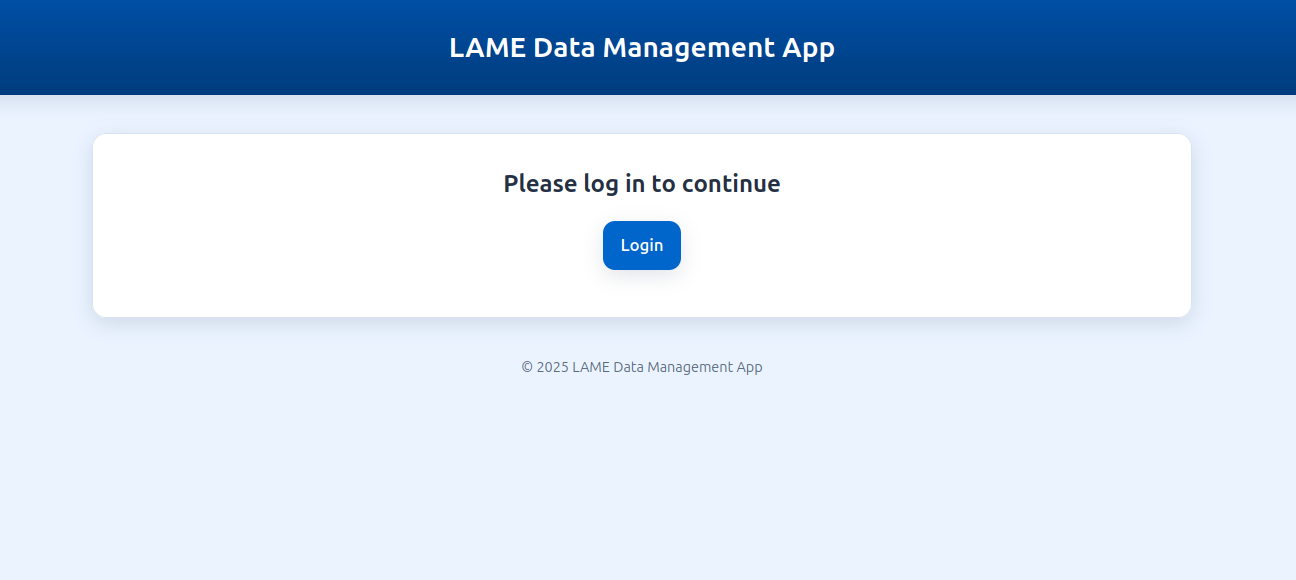
\includegraphics[width=0.9\textwidth]{img/chpt5/ui_login.png}
	\caption{Initial login screen of the LAME Data Management App.}
	\label{fig:ui-login}
\end{figure}

\begin{figure}[!h]
	\centering
	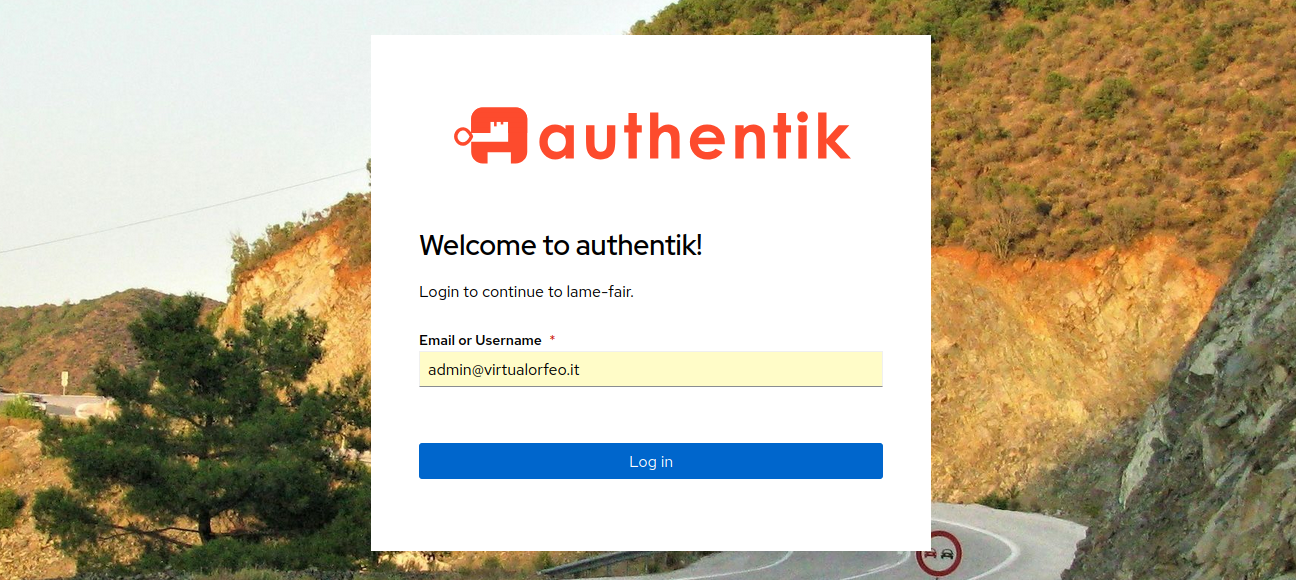
\includegraphics[width=0.9\textwidth]{img/chpt5/ui_authentik.png}
	\caption{Authentication via Authentik using OpenID Connect.}
	\label{fig:ui-authentik}
\end{figure}

\FloatBarrier
After successful login, users are taken to the dashboard (Figure~\ref{fig:ui-dashboard}), 
which acts as an entry point to the management board and other functions. 
If no proposals have been created yet, the board appears empty 
(Figure~\ref{fig:ui-empty-board}).

\begin{figure}[!h]
	\centering
	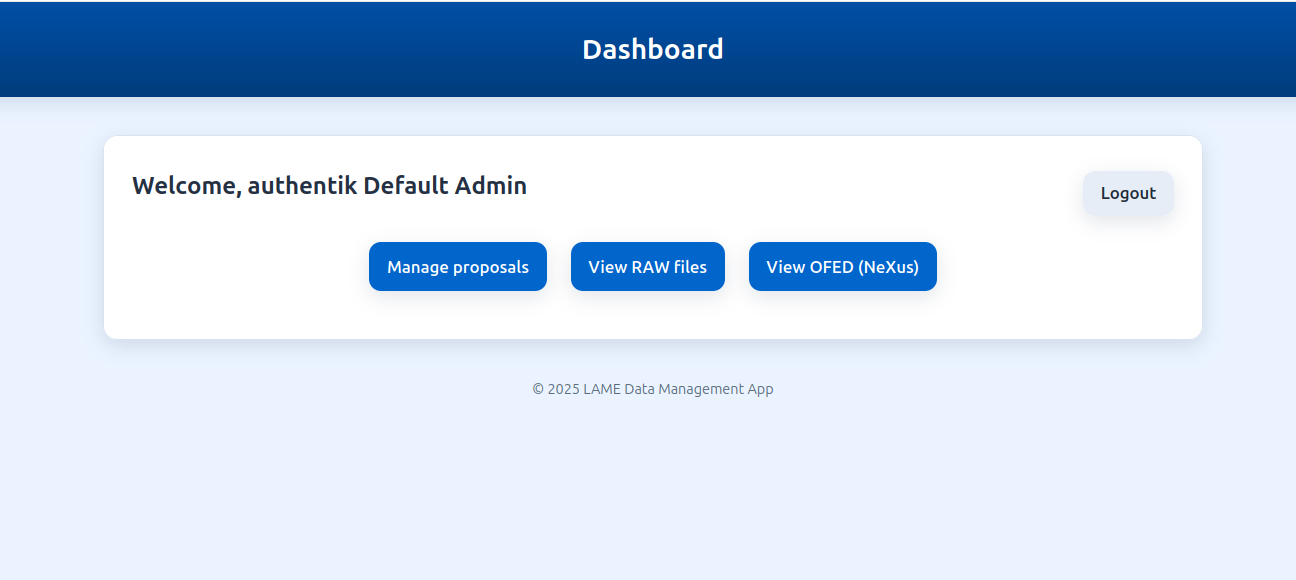
\includegraphics[width=0.9\textwidth]{img/chpt5/ui_dashboard.png}
	\caption{Dashboard view after successful login, showing navigation options.}
	\label{fig:ui-dashboard}
\end{figure}

\begin{figure}[!h]
	\centering
	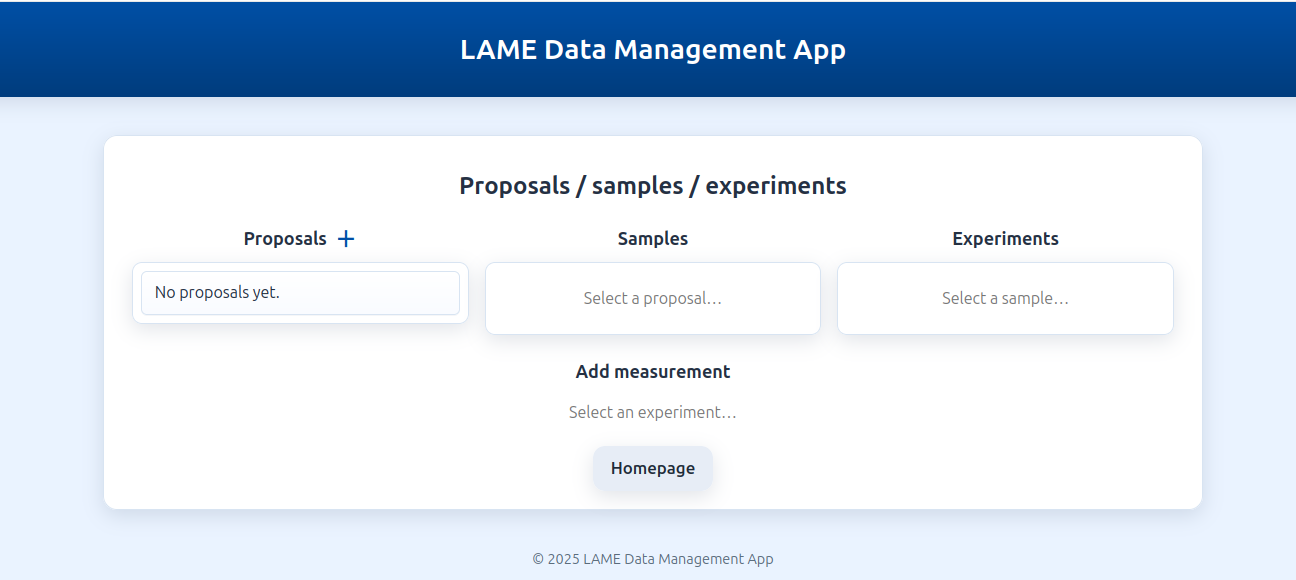
\includegraphics[width=0.9\textwidth]{img/chpt5/ui_empty_board.png}
	\caption{Management board before any proposals are created.}
	\label{fig:ui-empty-board}
\end{figure}

\FloatBarrier
New proposals are created via modal dialogs. 
Figure~\ref{fig:ui-modal-proposal} shows the form for entering the proposal number, 
principal investigator, and description. 
Once submitted, the new proposal appears in the left pane of the management board, 
and its details can be inspected as shown in Figure~\ref{fig:ui-proposal-info}.

\begin{figure}[!h]
	\centering
	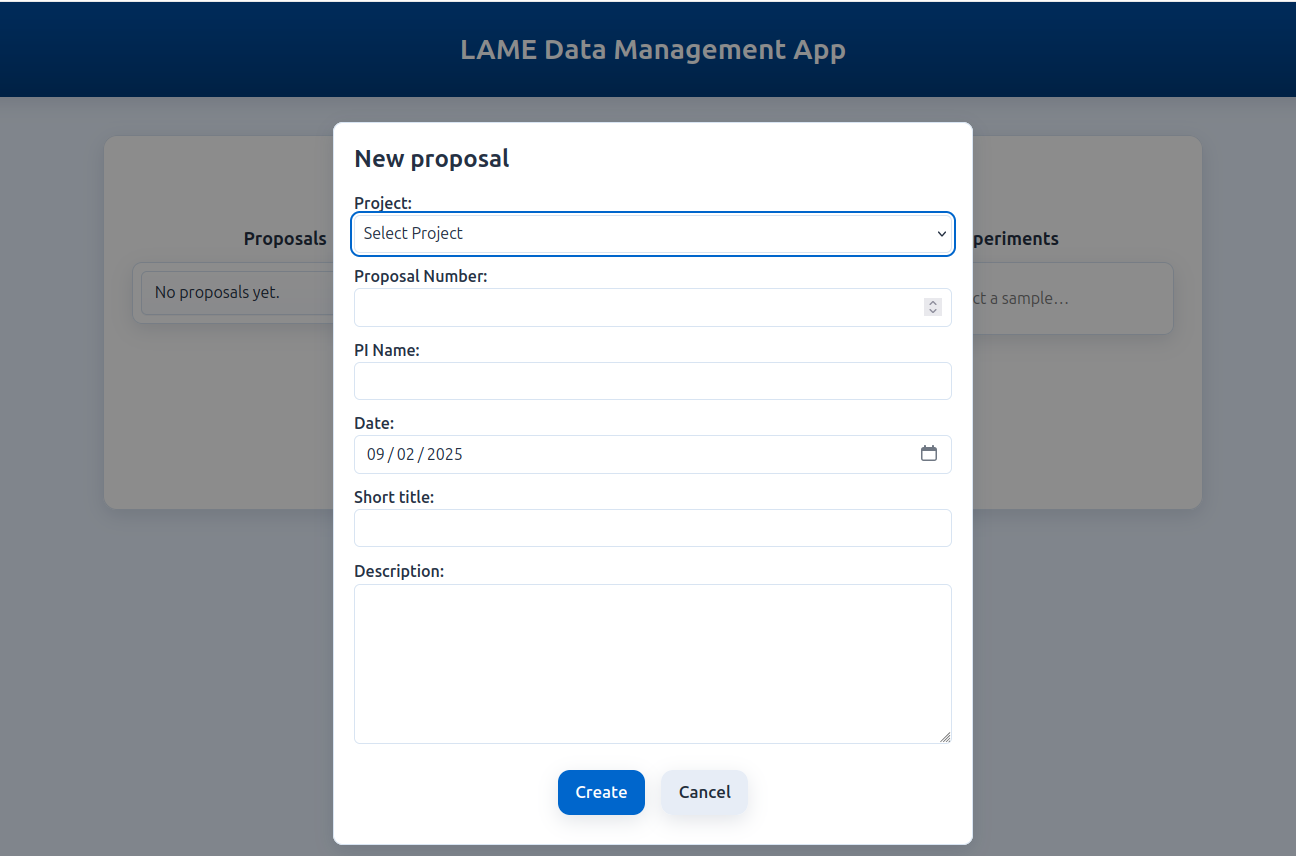
\includegraphics[width=0.9\textwidth]{img/chpt5/ui_modal_new_proposal.png}
	\caption{Modal form for creating a new proposal.}
	\label{fig:ui-modal-proposal}
\end{figure}

\begin{figure}[!h]
	\centering
	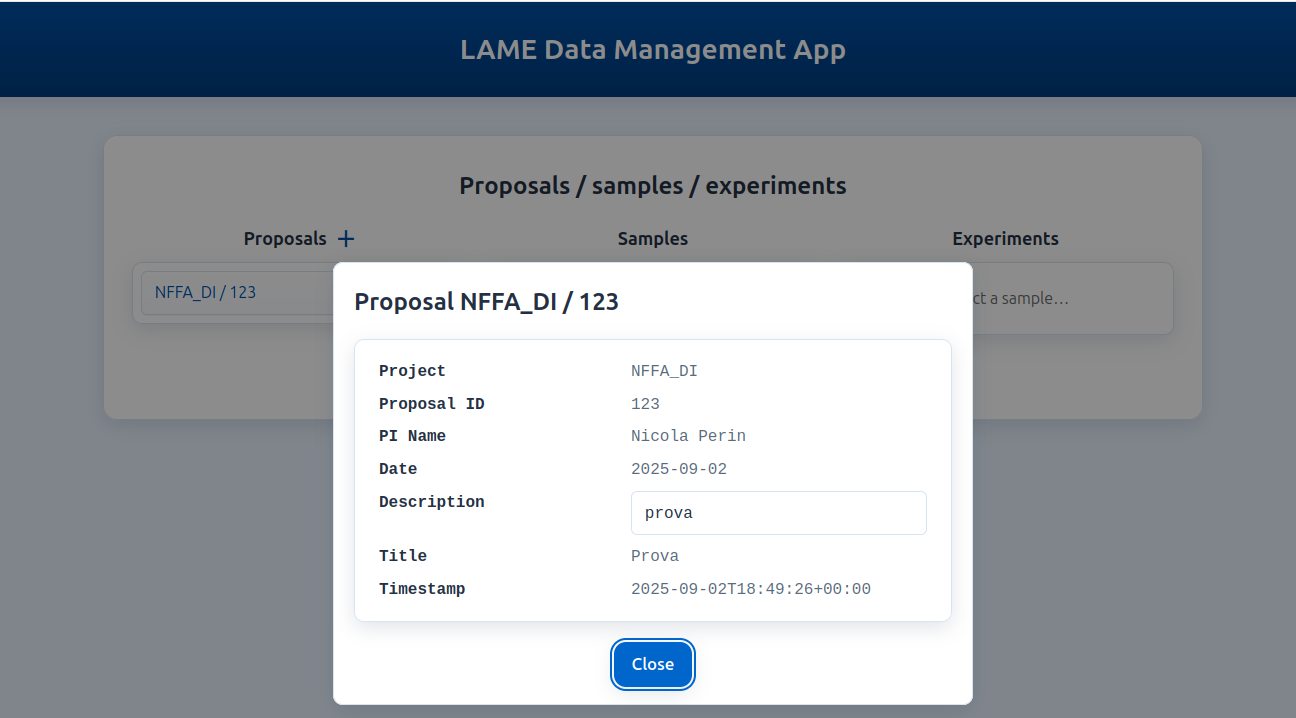
\includegraphics[width=0.9\textwidth]{img/chpt5/ui_proposal_info.png}
	\caption{Viewing details of a created proposal.}
	\label{fig:ui-proposal-info}
\end{figure}

\FloatBarrier
Within a proposal, users can register samples. 
The modal in Figure~\ref{fig:ui-modal-sample} allows adding a new sample with 
its metadata. 
Measurements can then be attached to experiments within each sample. 
Figure~\ref{fig:ui-add-measurement} shows the interface for creating a measurement entry, 
which is then linked to raw data files.

\begin{figure}[!h]
	\centering
	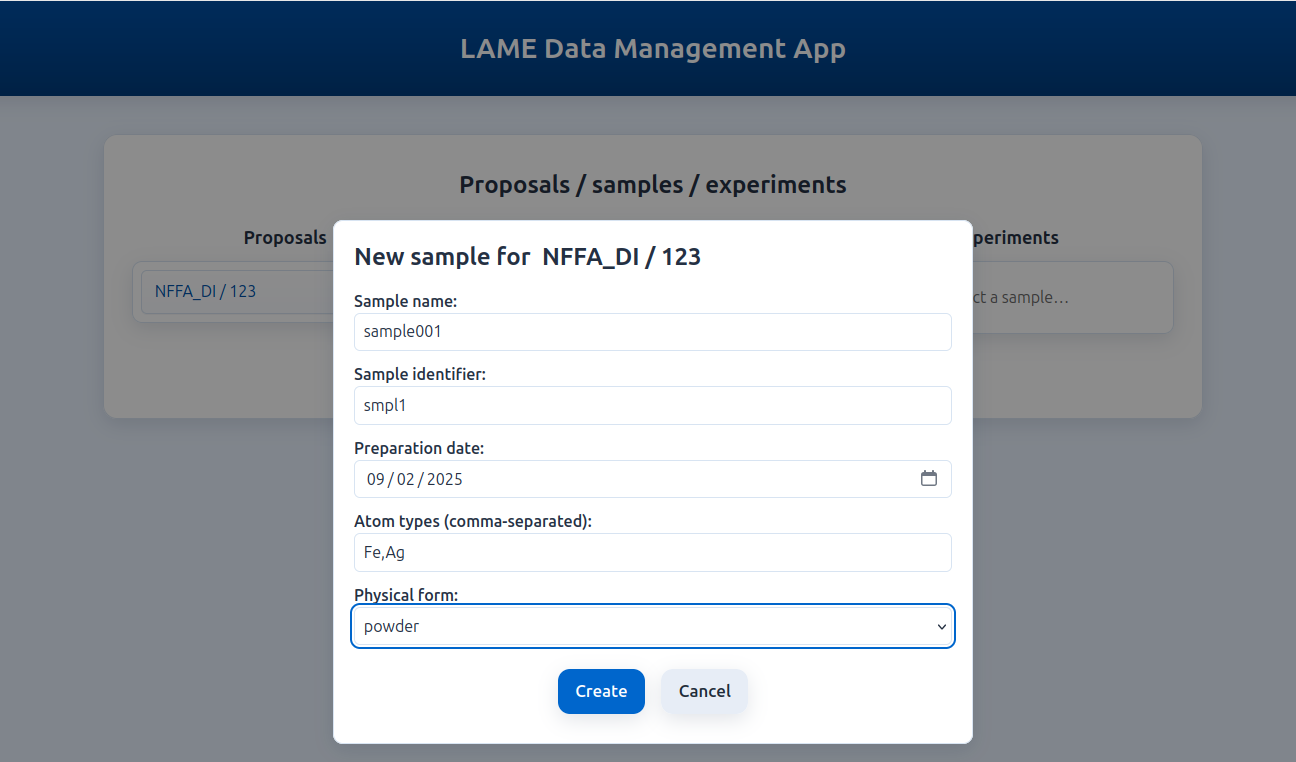
\includegraphics[width=0.9\textwidth]{img/chpt5/ui_modal_new_sample.png}
	\caption{Modal form for creating a new sample within a proposal.}
	\label{fig:ui-modal-sample}
\end{figure}

\begin{figure}[!h]
	\centering
	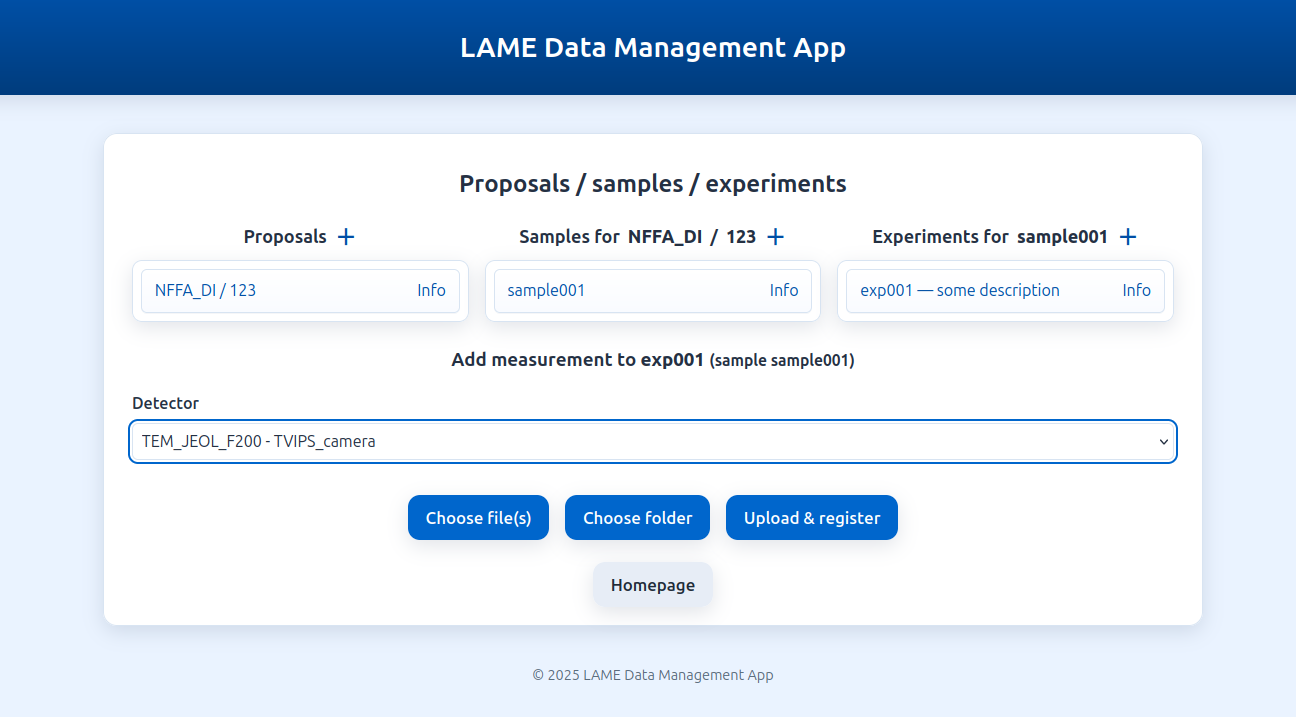
\includegraphics[width=0.9\textwidth]{img/chpt5/ui_add_measurement.png}
	\caption{Adding a new measurement under a sample and experiment.}
	\label{fig:ui-add-measurement}
\end{figure}

\FloatBarrier
Raw data, typically TIFF images, is uploaded through a drag-and-drop interface 
(Figure~\ref{fig:ui-file-picker}). 
Files are sent directly to object storage using presigned URLs, 
ensuring efficient transfer without passing through the Django server.

\begin{figure}[!h]
	\centering
	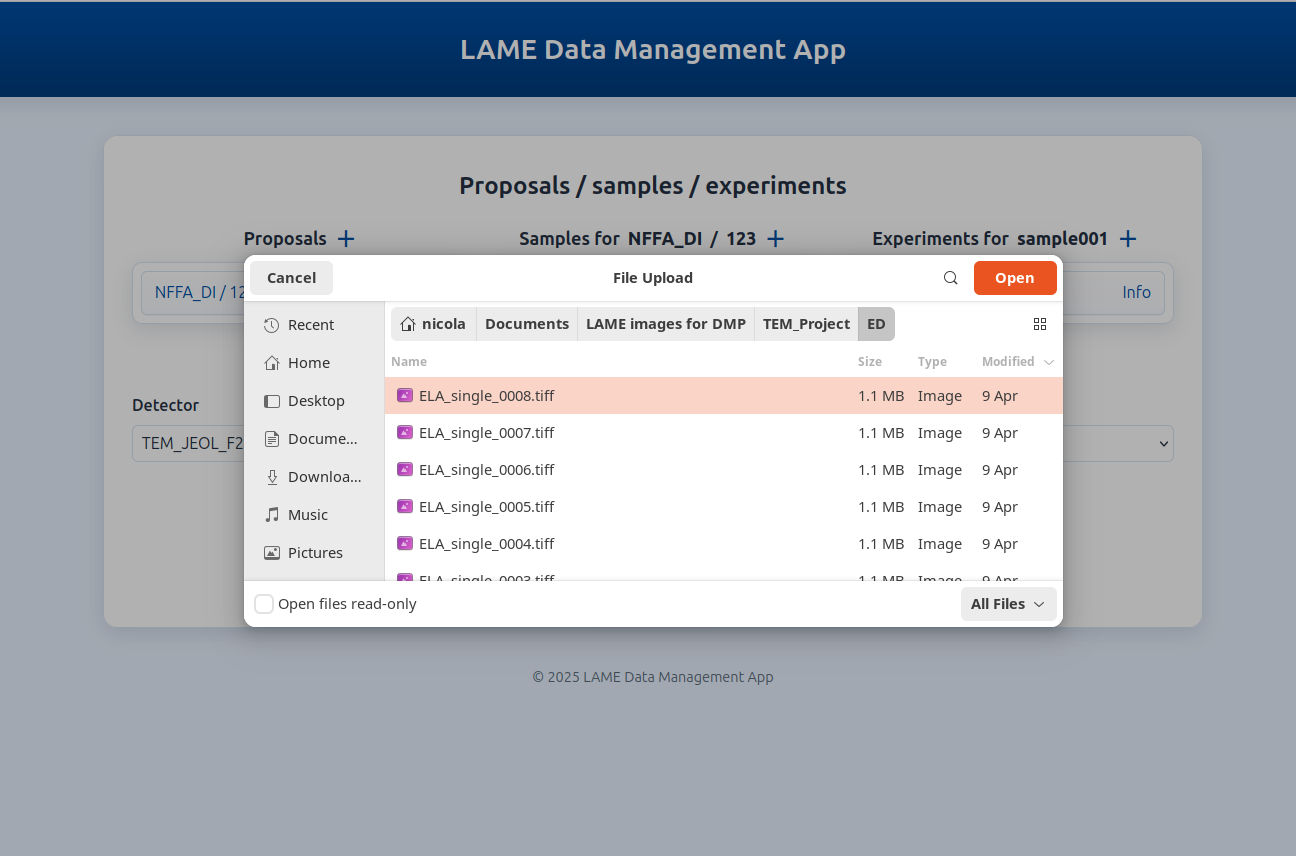
\includegraphics[width=0.9\textwidth]{img/chpt5/ui_file_picker.png}
	\caption{Selecting TIFF files for upload from the local filesystem.}
	\label{fig:ui-file-picker}
\end{figure}

\FloatBarrier
Once data is uploaded, users can browse it in the bucket view. 
At the top level, proposals are listed with their associated storage buckets 
(Figure~\ref{fig:ui-bucket-top}). 
Drilling down, users can see the files belonging to a specific experiment 
(Figure~\ref{fig:ui-bucket-experiment}), 
with options to download individual files, stream a ZIP archive, or generate 
aria2 manifests for high-throughput transfers.  

The same browsing interface is available for the “OFED” (derived data) view, 
which mirrors the raw data layout but contains NeXus files generated from 
the uploaded TIFFs. Because its appearance is identical to the raw data browser, 
we omit a separate screenshot here.

\begin{figure}[!h]
	\centering
	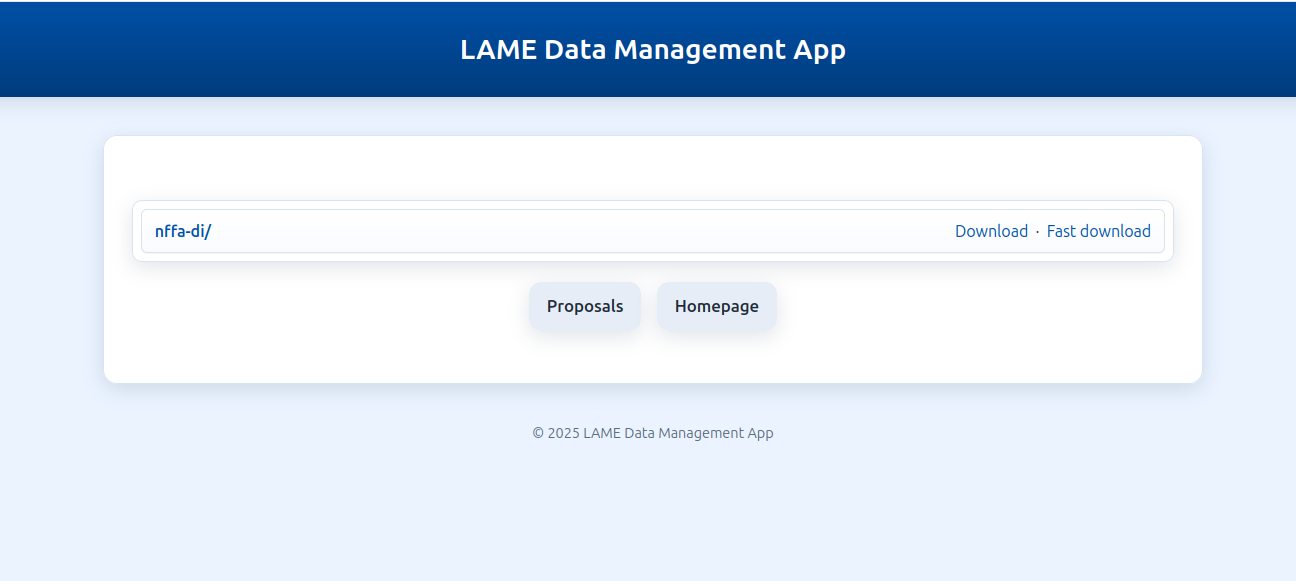
\includegraphics[width=0.9\textwidth]{img/chpt5/ui_bucket_top.png}
	\caption{Top-level view of available proposals in the bucket browser.}
	\label{fig:ui-bucket-top}
\end{figure}

\begin{figure}[!h]
	\centering
	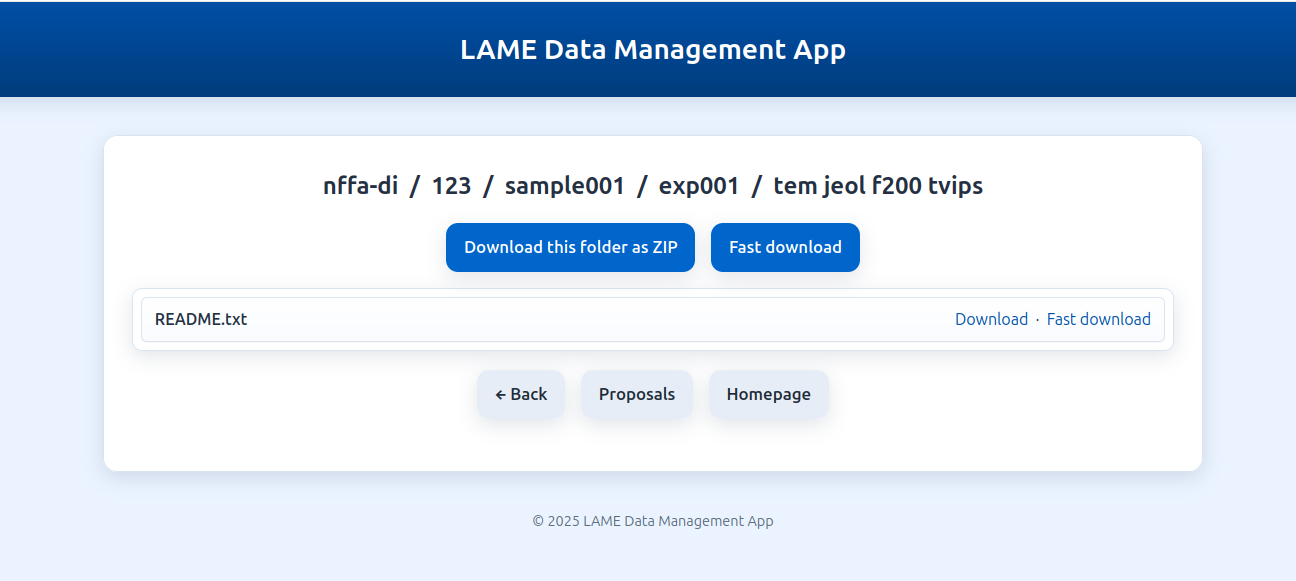
\includegraphics[width=0.9\textwidth]{img/chpt5/ui_bucket_experiment.png}
	\caption{Browsing files inside a specific experiment folder, with options for ZIP or fast download.}
	\label{fig:ui-bucket-experiment}
\end{figure}


%%%%%%%%%%%%%%%%%%%%%%%%%%%%%%%%%%%%%%%%%%%%%%%%%%%%%%%%%%%%%%%%%%%%%%%%%%%%%%%%%%%%%%%%%%
\FloatBarrier
\section{Security model in-app}\label{sec:security}

\paragraph{Authentication and login.}
The application never manages passwords itself. Instead, it delegates login to 
an external identity provider (Authentik) using OpenID Connect (OIDC).  
When a user tries to log in, they are redirected to Authentik.  
After successful login, Authentik returns an ID token (a signed JWT) which 
the app validates. From this token, a normal Django session is created.  
Logout also goes through OIDC: the app passes an ID token hint and a 
post-logout redirect so that both the identity provider and the local session 
are closed at the same time.

\paragraph{Claims and group mapping.}
Each token from Authentik carries \emph{claims}\footnote{OIDC claims are 
	fields embedded in the ID token, such as username, first/last name, or group 
	membership.}. The custom backend (\texttt{LameOIDCBackend} in 
\texttt{auth\_backends.py}) reads these claims and synchronizes them into the 
Django user model:
\begin{itemize}
	\item \texttt{preferred\_username} → \texttt{user.username},  
	\item \texttt{given\_name} / \texttt{family\_name} → \texttt{first\_name} and \texttt{last\_name},  
	\item \texttt{groups} → Django group membership (created on demand if missing).  
\end{itemize}
This way, group membership defined in Authentik or FreeIPA flows into Django 
and can be reused for permission checks.

\paragraph{Authorization rules.}
Access control in views builds on this group information:
\begin{itemize}
	\item \texttt{@login\_required} ensures that only authenticated users 
	can reach sensitive endpoints.  
	\item \texttt{@user\_passes\_test(is\_boss)} marks administrator-only 
	actions; \texttt{is\_boss} checks whether the user belongs to the right group.  
\end{itemize}
Dangerous operations such as bucket recreation, access to mirrored views, 
or management dashboards are strictly limited to admins.  
For normal data, each Proposal stores a \texttt{created\_by} reference 
so that ownership and provenance remain visible.

\paragraph{Protecting data transfers.}
Uploads and downloads rely on presigned S3 URLs.  
Each presigned URL is valid only for:
\begin{itemize}
	\item a single object (by key),  
	\item a single method (GET or PUT),  
	\item and a limited lifetime (usually one hour).  
\end{itemize}
Buckets are configured with strict CORS rules so that browsers can use these 
URLs only from the expected frontend origin.  
Sensitive secrets (S3 keys, OIDC client secrets, CA bundles) are never baked 
into container images. They are mounted as Kubernetes Secrets and injected at 
runtime. TLS checks are pinned to the internal FreeIPA CA by setting 
\texttt{AWS\_CA\_BUNDLE} and letting boto3/requests pick it up.

\paragraph{Recording what happened.}
Every uploaded file is checksummed in the background.  
The resulting SHA-256 digests are stored in the 
\texttt{MeasurementFileChecksum} table, ensuring that each file has a 
permanent fingerprint.  
Alongside the files, plain-text README files describe who created what, when, 
and with which description.  
Logs capture all major events — such as scheduling or finishing background 
jobs — together with the job ID and storage location.  
This combination of checksums, README files, and logs makes it possible 
to trace back the history of data and verify its consistency over time.


%%%%%%%%%%%%%%%%%%%%%%%%%%%%%%%%%%%%%%%%%%%%%%%%%%%%%%%%%%%%%%%%%%%%%%%%%%%%%%%%%%%%%%%%%%%

\section{Performance and scalability}\label{sec:performance}

\paragraph{Separating upload from conversion.}
Large files are never sent through the Django server itself.  
When a user uploads, the browser first asks the backend for a \emph{presigned URL}\footnote{A presigned URL is a temporary web address that allows the browser to upload or download a specific object from S3 directly, without passing the data through the application server.}.  
The browser then sends the file straight to S3/MinIO.  
The only parts that go through the Django server are very small: the request for the presigned URL (\texttt{/s3\_presign}) and the follow-up registration of metadata.  
Expensive work like computing checksums, converting TIFFs into NeXus files, and copying objects into mirror buckets runs later in background workers, not during the upload.  
This way, web responsiveness and heavy processing can scale independently.

\paragraph{Handling many things at once.}
\begin{itemize}
	\item \textbf{Uploads:} The Uppy\footnote{\url{https://uppy.io/}, a JavaScript library for drag-and-drop uploads with retries and progress bars.} uploader can open several parallel connections at once.  
	Object storage systems like Ceph RGW or MinIO are built to handle concurrent input/output, so the bottleneck is usually the network link, not the application.  
	Since Django never touches the file bytes, its CPU and memory stay stable even under heavy uploads.  
	
	\item \textbf{Workers:} Background work is handled by Redis Queue (RQ)\footnote{RQ (\url{https://python-rq.org/}) is a Python library that uses Redis as a queue to manage jobs.}.  
	Operators can start as many worker processes as needed.  
	Each worker can compute checksums or build NeXus files in parallel.  
	A stable job identifier is used so that if two requests try to process the same TIFF, only one job is actually run.  
	
	\item \textbf{Downloads:} For reading data, browsers again receive presigned URLs and fetch files directly from S3.  
	For folder downloads, the app streams a ZIP file on the fly.  
	Streaming means the server never holds the whole ZIP in memory: it sends each chunk as it is produced, letting the browser apply back-pressure\footnote{Back-pressure is when the receiving side slows down the sending side so that buffers do not overflow.}.
\end{itemize}

\paragraph{Database performance.}
The database tables enforce uniqueness (for example, one proposal number per project, one sample per proposal).  
Django automatically creates the necessary indexes to support these constraints.  
Extra indexes can be added for frequent lookups, such as checksums (\texttt{MeasurementFileChecksum(bucket, key)}).  
To avoid unnecessary database queries, list views use \texttt{select\_related}, which fetches related rows in a single query.

\paragraph{Where caching helps.}
\begin{itemize}
	\item \textbf{UI fragments:} Proposal and sample lists can be cached for a short time, which reduces the load when users rapidly switch panes in the HTMX interface.  
	\item \textbf{Presigned URLs:} These should not be cached on the server side, because they expire quickly and are tied to a specific file.  
	Clients, however, may reuse them during multi-file uploads.  
	\item \textbf{README parsing:} When a modal needs to display a README file, it can cache the parsed lines until the file changes (detected via its ETag\footnote{An ETag is an identifier provided by the storage service that changes whenever the file content changes.}).  
\end{itemize}

\paragraph{Network and TLS security.}
All S3 clients are configured to use TLS certificates from a trusted CA bundle\footnote{A Certificate Authority (CA) bundle is a set of trusted certificates used to verify secure connections.}.  
This bundle is mounted at runtime as a Kubernetes Secret, not embedded in the image.  
For the application endpoints, TLS termination is handled by Ingress\footnote{Ingress is a Kubernetes component that manages external access to services, often with TLS termination.} in combination with MetalLB\footnote{MetalLB is a Kubernetes load-balancer implementation for bare-metal clusters.}.  
Presigned URLs point at S3/MinIO with HTTPS, so encryption holds end-to-end.

\paragraph{Dealing with failures.}
The S3 client is configured to retry failed requests a few times before giving up.  
Background jobs also use retry policies with exponential backoff, and they are written to be safe to run multiple times without causing duplicates or corruption.  
If a bucket does not exist, the code can recreate it and reapply its CORS configuration.  
The \texttt{/buckets/} view shows clear error messages when something is missing, and administrators can fix it with one click.

\paragraph{Scaling in operations.}
Web processes and background workers can scale separately.  
The main scaling factor is storage: moving from local volumes to a CSI-backed block store\footnote{CSI (Container Storage Interface) is a standard for connecting Kubernetes to different storage systems.} or to an external S3 cluster requires no code change because everything goes through the storage gateway abstraction.  
Redis can be replaced by a managed service if needed; RQ workers keep working the same way.  
The API and UI servers are stateless (except for the shared database), which means they can be horizontally scaled behind the load balancer without special coordination.


\bigskip

\noindent\textbf{Summary.}
This chapter takes a detailed look at the Django application for managing experimental data. The system organizes projects, proposals, samples, and experiments in a clear hierarchy, with each creation automatically writing metadata into S3 buckets alongside the raw data. Large microscope outputs are uploaded directly to object storage through presigned URLs, keeping the web server light, while background workers handle heavier jobs like checksums and NeXus conversions. Metadata from TIFFs is translated into standardized NeXus structures using JSON mapping files, making the system adaptable across instruments. All storage operations go through a thin gateway layer that hides S3 details and simplifies testing. A REST API exposes the same functionality available in the browser-based management board, which uses HTMX modals for interactive creation and error handling. Authentication is delegated to Authentik via OIDC, group claims control authorization, and presigned URLs enforce strict, time-limited access. Checksums, READMEs, and logs together provide a consistent record of data handling. Finally, the architecture separates uploads from processing, allows workers and web processes to scale independently, and ensures resilience through retries and safe replays, making the platform both robust and scalable for growing data needs.
